\documentclass[a4paper,12pt]{article}

\usepackage{ProfModels}

 
\begin{document}

\begin{Maquette}[DM]{Prive=false, Numero=4, Niveau=1, Date=\today}

\begin{exercice}
\begin{enumerate}
\item Compléter les expressions par qui convient :
$$
 8x = 2x + \cdots\quad ;; \quad
 14xy = 2x \times \cdots\quad ;; \quad
 146 ab = 200 ab - \cdots\quad ;; \quad
 52 x = 12 x + \cdots
$$
\item Réduire ce qui suit :
$$
3x+2+6x-7\quad ;; \quad
5ab-1+3ab-8-14ab\quad ;; \quad
6a^{2}+a-3a^{2}-5a+4
$$
\item Développer et réduire les produits suivants:
$$
-7x(2x+1)\quad ;; \quad
5ab(2ab+3a-8b)\quad ;; \quad
(2x+4)(5x+8)\quad ;; \quad
(6x-7)(5x-2)
$$
\item Factoriser :
$$
8x-8y\quad ;; \quad
25ab+5\quad ;; \quad
49x^{2}+56y^{3}
$$
\end{enumerate}
\end{exercice}

\begin{exercice}
Résoudre les équations suivantes :
$$
x+4=2\quad ;; \quad
7+a=-3\quad ;; \quad
-4-x=1
$$
$$
2+x=-x+1\quad ;; \quad
3x-5=6\quad ;; \quad
4(3x-1)=2x-3
$$
$$
-2x+6=-4x-8\quad ;; \quad
12b-1=5b-17\quad ;; \quad
-7a-9=-15-a
$$
\end{exercice}
\begin{exercice}
\begin{tikzpicture}
\tkzDefPoints{0/0/A,5/0/B,5/3/C,0/3/D}
\tkzDrawSegments(A,B B,C C,D D,A)

\tkzLabelPoint[left](A){A}
\tkzLabelPoint[below right=5pt](B){B}
\tkzLabelPoints[above](C,D)
\tkzDrawSegment[dim={$x$,-0.5cm,below=5pt}](A,B)
\tkzDrawSegment[dim={$y$,0.3cm,right=5pt}](C,B)

\end{tikzpicture}
\end{exercice}
\end{Maquette}
\end{document}